% phpcpd-next — academic paper
% Build: bash bin/build-paper.sh   (or: pdflatex paper.tex ; pdflatex paper.tex)
%
% STYLE CONVENTIONS (keep consistent when editing):
%   Prose  — Strunk & White: omit needless words, active voice, parallel lists,
%            precise diction (no slang).
%   Numbers — Chicago Manual of Style 16.10 alternative (technical) rule:
%            * spell out single-digit counts in running prose (two methods, six corpora);
%            * use numerals for 10 and above, and within a category keep them
%              consistent (e.g. "17 ... to 0");
%            * always numerals for percentages, measurements, math-mode quantities,
%              edit-distance costs/budgets, CLI literal values, versions, table data,
%              and designators (Type-3, level 10, R1, v6.0.3);
%            * never begin a sentence with a numeral.
\documentclass[10pt,a4paper]{article}

\usepackage[utf8]{inputenc}
\usepackage[T1]{fontenc}
\usepackage{lmodern}
\usepackage[margin=1in]{geometry}
\usepackage{amsmath,amssymb}
\usepackage{booktabs}
\usepackage{multirow}
\usepackage{makecell}
\usepackage{array}
\usepackage{xcolor}
\usepackage{caption}
\usepackage{subcaption}
\usepackage{listings}
\usepackage{enumitem}
\usepackage{titlesec}
\usepackage{microtype}
\usepackage{pgfplots}
\pgfplotsset{compat=1.16}
\usepgfplotslibrary{statistics}
\usetikzlibrary{patterns}

% ---- monochrome palette: grayscale shades for figures, one tone for links ----
\definecolor{g1}{gray}{0.00}
\definecolor{g2}{gray}{0.35}
\definecolor{g3}{gray}{0.60}
\definecolor{g4}{gray}{0.82}
\definecolor{linkmono}{gray}{0.30}

\usepackage[colorlinks=true,allcolors=linkmono]{hyperref}

% ---- listings: uniform monospace, no syntax colouring (mono pattern throughout) ----
\lstset{
  basicstyle=\ttfamily,
  columns=fullflexible,
  keepspaces=true,
  breaklines=true,
  breakatwhitespace=true,
  showstringspaces=false,
  frame=single,
  framesep=4pt,
  rulecolor=\color{black!35},
}

% lightweight theorem-like environments without amsthm dependency
\newcounter{defn}[section]
\newcommand{\defn}[1]{\par\medskip\refstepcounter{defn}%
  \noindent\textbf{Definition~\thedefn} (#1)\textbf{.}\ }
\newcounter{prop}[section]
\newcommand{\prop}[1]{\par\medskip\refstepcounter{prop}%
  \noindent\textbf{Proposition~\theprop} (#1)\textbf{.}\ \itshape}
\newcounter{lem}[section]
\newcommand{\lem}[1]{\par\medskip\refstepcounter{lem}%
  \noindent\textbf{Lemma~\thelem} (#1)\textbf{.}\ \itshape}

\titleformat{\section}{\large\bfseries}{\thesection}{0.6em}{}
\titleformat{\subsection}{\normalsize\bfseries}{\thesubsection}{0.6em}{}

\setlength{\parskip}{2pt}
\setlength{\parindent}{1.2em}
% absorb minor overfulls from long unbreakable code identifiers
\setlength{\emergencystretch}{3em}

\title{\textbf{Token-Based Clone Detection for PHP:\\
An Empirical Evaluation of Methods and a Labelled Benchmark}}

\author{Luciano Federico Pereira\\[2pt]
\small ORCID: \href{https://orcid.org/0009-0002-4591-6568}{0009-0002-4591-6568}}

\date{June 2026}

\begin{document}
\maketitle

\begin{abstract}
\noindent
\texttt{phpcpd} is a widely used PHP copy/paste detector whose last released version (6.0.3, 2020)
performs Rabin--Karp exact matching of Type-1 and Type-2 clones. A subsequent, unreleased 7.0.0
development line added a ConQAT-style approximate suffix-tree algorithm for Type-3 (near-miss)
detection (contributed upstream as pull request~\#199); however, 7.0.0 was never released and the
project was archived in 2023, so this capability did not reach users. The clone-detection literature
offers further methods --- order-invariant token-bag matching and type-aware normalization --- that
had not been applied to PHP, and, unlike Java (BigCloneBench) or C (POJ-104), no labelled PHP clone
benchmark existed on which to evaluate any of them. This paper reports an empirical study based on the
archived \texttt{phpcpd} codebase. We (i)~modernize it reproducibly to PHP~8.5, PHPStan level~10, and a
159-test suite, and complete and evaluate its previously unreleased suffix-tree engine; (ii)~implement
additional literature-grounded methods as selectable engines --- a SourcererCC token-bag matcher,
type-aware edit weights, a token-type abstraction with a \texttt{-{}-type-anchored} variant, an IDF
stopword filter, and an incremental index that provably reproduces a full pass; and (iii)~construct
\textbf{BCB-PHP}, a labelled PHP clone benchmark (to our knowledge the first), comprising a
mutation-injection harness over a pinned, six-corpus type-density gradient. Evaluating each method on
BCB-PHP yields a type-density$\times$clone-density map, a specificity increase of $+10.9$ to $+45.3$
points from type-anchored normalization at no recall cost, and confirmed inconsistent clones in an
application corpus. The results motivate a combined exact-and-reorder-tolerant default configuration
(\texttt{rk+tb}); identifier fuzzing is shown to reduce precision substantially, and approximate
suffix-tree matching to be better suited to targeted analysis than to default use. BCB-PHP is released
for reuse; its type-density gradient supports further study of clone detection on modern typed versus
traditional untyped PHP and of differences between methods.
\end{abstract}

\section{Introduction}

\texttt{phpcpd} is a carefully engineered PHP copy/paste detector developed by Sebastian Bergmann: a
Rabin--Karp rolling hash over a normalized token stream that hashes fixed windows, reports collisions,
and detects Type-1 and Type-2 clones. It is fast, dependency-light, and widely used. Its last released
version, 6.0.3 (2020), implements this single Rabin--Karp strategy and does not attempt Type-3
(near-miss/gapped) or reorder-tolerant detection --- an appropriate scope for an exact-match detector.

A subsequent development line did go further: an unreleased 7.0.0 added a ConQAT-style approximate
suffix-tree algorithm with a configurable edit budget for Type-3 detection~\cite{conqat}, contributed
upstream as pull request~\#199. That release, however, was never published --- its changelog entry
carries an unfilled date --- and the repository was archived in 2023, so the capability remained in the
codebase but absent from any release and unevaluated in practice. The clone-detection literature offers
further methods still: SourcererCC's order-invariant token-bag matching for reordered
code~\cite{sourcerercc} and Toma's token-type abstraction for stronger Type-2
normalization~\cite{toma}, neither of which had been applied to PHP. Evaluating any of these on PHP
faced a further obstacle: unlike Java (BigCloneBench~\cite{bigclonebench}) or C (POJ-104), no labelled
PHP clone benchmark existed.

\paragraph{Approach.} Building on the archived \texttt{phpcpd} codebase, we modernize it, complete and
evaluate its previously unreleased suffix-tree engine, implement additional literature-grounded
methods, and construct the benchmark required to evaluate them. We then determine empirically which
methods are appropriate for a default configuration in a fast command-line tool. The evaluation
indicates that a combined exact-and-reorder-tolerant configuration is the most suitable default, that
identifier fuzzing substantially reduces precision, and that approximate suffix-tree matching is better
reserved for targeted analysis.

\paragraph{Contributions.}
\begin{enumerate}[leftmargin=1.4em,itemsep=1pt,topsep=2pt]
  \item A \textbf{diff-level reproducible modernization} of an archived PHP tool to PHP~8.5, PHPStan
        level~10, PER-CS~2.0, and a 159-test suite, including the completion and first evaluation of
        \texttt{phpcpd}'s previously unreleased ConQAT suffix-tree engine (\S\ref{sec:method}).
  \item \textbf{Five detection methods implemented} as selectable engines on the inherited base: a
        SourcererCC token-bag matcher with IDF filtering, type-aware edit weights, an extended
        token-type abstraction with a type-anchored variant, inconsistent-clone reporting, and an
        incremental index --- each tied to a primary reference and an end-to-end test
        (\S\ref{sec:methods},~\S\ref{sec:engineering}).
  \item \textbf{BCB-PHP, a labelled PHP clone benchmark} (to our knowledge the first): a
        mutation-injection harness over a pinned, six-corpus type-density gradient (\S\ref{sec:eval}),
        released for reuse --- its gradient supports further study of modern typed vs.\ traditional
        untyped PHP and of method
        differences.
  \item An \textbf{empirical evaluation} on BCB-PHP yielding a type-density$\times$clone-density map, a
        $+10.9$ to $+45.3$ point specificity lift from type-anchored normalization at zero recall cost,
        a six-corpus method comparison, and real inconsistent clones in an application corpus
        (\S\ref{sec:eval}) --- from which we recommend the \texttt{rk+tb} default (\S\ref{sec:practical}).
\end{enumerate}

\section{Background: the phpcpd Codebase and Its Detection Methods}
\label{sec:methods}

\subsection{The released base engine (Rabin--Karp)}
phpcpd's last released version (6.0.3) provides a single strategy, \texttt{DefaultStrategy}, a
Rabin--Karp matcher. It normalizes tokens (whitespace and comments stripped; \texttt{-{}-fuzzy}
rewrites \lstinline!T_VARIABLE! to a placeholder), builds a per-token rolling signature, hashes fixed
windows of \texttt{-{}-min-tokens} tokens, and reports colliding windows filtered by
\texttt{-{}-min-lines}. It detects Type-1 and Type-2 exact-match clones and, by construction, tolerates
neither gaps nor reordering.

\subsection{The inherited suffix-tree engine (unreleased 7.0-dev)}
The repository's unreleased 7.0.0 line, which we fork, introduces a second strategy through a selector
in \texttt{Application.php} (upstream code; \texttt{tokenbag} is the only branch we add):

\begin{lstlisting}[basicstyle=\ttfamily\small]
return match ($algorithm) {                               // selector: upstream 7.0-dev
    null, 'rabin-karp' => new DefaultStrategy($config),    // phpcpd base engine
    'suffixtree'       => new SuffixTreeStrategy($config),  // upstream, PR #199
    'tokenbag'         => new TokenBagStrategy($config),    // added in phpcpd-next
};
\end{lstlisting}

The \texttt{SuffixTreeStrategy} $\rightarrow$ \texttt{ApproximateCloneDetectingSuffixTree} (an
implementation of the ConQAT algorithm~\cite{conqat}, contributed upstream as PR~\#199) tokenizes into
an \texttt{AbstractToken[]} word, appends a sentinel, builds a generalized suffix tree, and in
\lstinline!findClones($minLength, $maxErrors, $headEquality)! compares candidate token sequences by
\emph{approximate} match. A Levenshtein edit-distance matrix \lstinline!edBuffer! is maintained over
token sequences; a candidate extends only while the running edit distance stays $\le$ \texttt{maxErrors}
(the \texttt{-{}-edit-distance} flag, default~5), and \texttt{headEquality} enforces an exact-match
prefix before edits are allowed, as in ConQAT. Comparing by edit distance rather than hash equality,
this method detects Type-3 (near-miss/gapped) clones: inserted, deleted, or substituted statements
within the edit budget are tolerated. Because 7.0.0 was never released, this engine had not been
evaluated; we modernize it (\S\ref{sec:method}), repair two latent defects it exposed
(\S\ref{sec:engineering}), and evaluate it (\S\ref{sec:eval}).

\defn{token edit distance}
For token sequences $a_{1..m}$, $b_{1..n}$, the matcher fills $D$ with
\[
D[i,j]=\min\!\begin{cases}
D[i\!-\!1,j]+1 & \text{(deletion)}\\
D[i,j\!-\!1]+1 & \text{(insertion)}\\
D[i\!-\!1,j\!-\!1]+c(a_i,b_j) & \text{(match/substitution)}
\end{cases}
\]
and reports a clone while $\min_k D[\cdot,k]\le \texttt{maxErrors}$. With uniform $c\equiv 1$ this is
plain Levenshtein; \S\ref{sec:engineering} (R2) replaces $c$ with a type-aware cost.

\lem{band sufficiency}
$D[i,j]\ge |i-j|$, so $|i-j| > \texttt{maxErrors}$ implies $D[i,j] > \texttt{maxErrors}$ and no
alignment of cost $\le \texttt{maxErrors}$ passes through $(i,j)$.\upshape\
\emph{Proof.} Aligning an $i$-token prefix with a $j$-token prefix requires at least $|i-j|$ insertions
or deletions, hence $D[i,j]\ge|i-j|$; the threshold and path claims follow. $\square$\ Consequently the
cells outside the band $|i-j|\le\texttt{maxErrors}$ cannot affect any reported clone, and computing only
the band --- $2\,\texttt{maxErrors}+1$ cells per diagonal over $L$ steps --- costs
$O(L\cdot\texttt{maxErrors})$ rather than $O(L^2)$ with identical output. This justifies the banded
optimization of \S\ref{sec:practical}.

\subsection{Methods added in phpcpd-next}
Beyond modernizing and evaluating the inherited engines, we contribute five methods grounded in the
literature: a SourcererCC token-bag matcher~\cite{sourcerercc}, type-aware edit weights, an extended
token-type abstraction~\cite{toma} with a type-anchored variant, inconsistent-clone reporting, and an
incremental index. Each is implemented behind a flag and pinned by an end-to-end test
(\S\ref{sec:engineering}). Two findings from the literature (\S\ref{sec:findings}) guide which methods
are appropriate by default, and the benchmark of \S\ref{sec:eval} decides it.

\subsection{Clone-type coverage}
Using the Roy \& Cordy taxonomy~\cite{roycordy} (Type-1 identical up to layout; Type-2 up to renamed
identifiers/literals/types; Type-3 near-miss/gapped; Type-4 semantic), Table~\ref{tab:coverage}
contrasts phpcpd's base engine with the methods phpcpd-next adds. Note on Type-2: phpcpd's
\texttt{-{}-fuzzy} abstracts only \lstinline!T_VARIABLE!; the shared \texttt{TokenNormalizer} we add
(R3) provides full Type-2 normalization under \texttt{-{}-fuzzy} for every method.

\begin{table}[h]
\centering
\caption{Clone-type coverage: phpcpd's base Rabin--Karp engine vs.\ the methods added in phpcpd-next.}
\label{tab:coverage}
\small
\begin{tabular}{c p{4.2cm} p{5.2cm}}
\toprule
\textbf{Type} & \textbf{phpcpd base (Rabin--Karp)} & \textbf{phpcpd-next (added methods)} \\
\midrule
1 & \checkmark & \checkmark \\
2 & partial (\texttt{-{}-fuzzy}, \lstinline!T_VARIABLE! only) & \checkmark\ (full, via \texttt{TokenNormalizer}) \\
3 & --- (exact hash) & \checkmark\ (suffix tree, edit dist.\ $\le$ \texttt{-{}-edit-distance}; token-bag for reorder) \\
4 & --- & --- \\
\bottomrule
\end{tabular}
\end{table}

\section{Two Literature Findings That Guide Method Selection}
\label{sec:findings}

\paragraph{Finding 1 --- simple clones dominate~\cite{toma}.} In real-world OSS most clones are
Type-1/2; Type-3 is a meaningful minority; Type-4 is rare. Approaches that sacrifice scalability to
chase Type-4 ``may not be practical in real life.'' For a fast CLI linter, \textbf{Type-3 is the
ceiling worth reaching; Type-4 is out of scope.}

\paragraph{Finding 2 --- the dangerous clones are \emph{inconsistent} ones~\cite{conqat}.} Bug risk
concentrates where one copy of a near-miss clone was patched and its sibling was not. The value of
Type-3 detection is therefore not recall for its own sake but \textbf{surfacing diverging copies}.

\paragraph{Joint implication.} The methods worth adding are those that make Type-3 detection
\emph{better, faster, and usable by default for bug-hunting} --- approximate and reorder-tolerant
matching with inconsistency reporting --- not neural Type-4 machinery. These two findings set the
selection criterion the benchmark then applies.

\section{Modernization Methodology}
\label{sec:method}

The revival is recorded diff-by-diff as a primary source (not retrospectively). The citable
methodology:
\begin{enumerate}[leftmargin=1.4em,itemsep=1pt,topsep=2pt]
  \item \textbf{Platform-first.} \texttt{composer.json} pins \texttt{platform.php = 8.5} so
        dependency incompatibilities surface at install time, not runtime.
  \item \textbf{Bugs before idioms.} Six genuine correctness fixes (an \lstinline!empty($object)!
        always-false guard; an unguarded \lstinline!preg_replace! null return; an
        \lstinline!averageSize()! division-by-zero; \lstinline!current()! on an empty array; \dots)
        landed \emph{before} any cosmetic modernization.
  \item \textbf{One idiom at a time}, each with a diff and a rationale: typed properties
        $\rightarrow$ \texttt{readonly class} $\rightarrow$ constructor promotion $\rightarrow$ typed
        constants $\rightarrow$ \texttt{\#[\textbackslash Override]} $\rightarrow$ PHPDoc generics.
  \item \textbf{Static analysis as a ratchet.} PHPStan driven $64\rightarrow0$ errors, then the
        level raised from~9 to \texttt{max} (level~10). The gate only tightens.
  \item \textbf{Dependency re-unification and decoupling.} The four \texttt{sebastian/*} runtime
        packages were replaced with owned code, giving a zero-runtime-dependency tool decoupled from
        the PHPUnit release train.
  \item \textbf{Tests last, and they paid off immediately.} The suite surfaced a latent bug invisible
        to static analysis: \lstinline!SuffixTreeStrategy::postProcess()! threw on an empty file
        list, a valid call path.
\end{enumerate}

\noindent\emph{Measured methodological claim:} the modernization reached PHPStan level~10 with zero
errors and \emph{still} harboured a latent runtime bug that only a test exercised --- a concrete data
point that static analysis and testing are complementary, not redundant.

\section{Methods Implemented and Evaluated}
\label{sec:engineering}

With the inherited suffix tree reaching Type-3 (\S\ref{sec:methods}), we examine its limitations and
add further methods. Each is implemented behind a flag and pinned by an end-to-end test;
Table~\ref{tab:roadmap} summarizes. The set is bounded by a marginal-returns criterion: a method is
admitted while the capability it adds outweighs its marginal cost in precision or runtime, and the
three methods for which that balance reverses (R6--R8) are declined rather than deferred.

\paragraph{A limitation of the suffix tree: intra-block reordering.} The suffix tree models a clone as
one approximately-matching \emph{contiguous} substring of a linearised token stream. A swapped pair of
statements looks like a delete followed by an insert --- two operations that consume at least~2 from
\texttt{maxErrors}; at the default budget of~5 a few reorderings exhaust it. A suffix tree on a
linear token stream \emph{cannot} be order-invariant within a block. A token-multiset
(bag-of-tokens) model is order-invariant by construction, which is why it complements the suffix tree
rather than duplicating it.

\defn{token-bag overlap clone (SourcererCC~\cite{sourcerercc})}
Represent each block as a token multiset. Blocks $A,B$ are clones iff their multiset intersection
satisfies
\[
|A\cap B|\ \ge\ \theta\cdot\max(|A|,|B|),\qquad \theta=0.7\ \text{by default,}
\]
computed via an inverted index (token $\rightarrow$ blocks). This is order-invariant: if $B$ is $A$
with two statements swapped, $A\cap B=A$ and the score is~1.

\defn{IDF stopword filter}
Let $N$ be the number of blocks and $\mathrm{df}(t)$ the number of blocks containing token~$t$.
A token is a \emph{stopword} (excluded from the index and from $|A\cap B|$) iff
\[
\frac{\mathrm{df}(t)}{N} > 0.6,\qquad N\ge 5.
\]
Under \texttt{-{}-fuzzy}, normalized placeholders (\lstinline!T_VARIABLE:$!, \lstinline!T_STRING:ID!)
occur in almost every PHP body and carry no discriminative power; removing them prevents
false-positive inflation. The filter is disabled below five blocks so micro-fixtures are unaffected.

Each method below is \textbf{implemented and tested}; Table~\ref{tab:roadmap} summarizes.

\paragraph{R1 --- token-bag $+$ inverted index $+$ IDF (SourcererCC).}
\lstinline!TokenBagStrategy! (selectable via \texttt{-{}-algorithm tokenbag}). Blocks are
function/method bodies (brace-tracked, no parser); clones are overlap pairs gathered through the
inverted index. \emph{Complementarity verified end-to-end:} a function with two statements swapped is
detected by the token bag while both Rabin--Karp and the suffix tree (\texttt{-{}-edit-distance 5})
miss it at min-tokens~25. \emph{Precision:} the IDF filter reduced a self-application scan of the tool's own
\texttt{src/} from 17 reported pairs (all false positives) to~0.

\paragraph{R2 --- type-aware edit weights.} \lstinline!SubstitutionCost! replaces the uniform
$c\equiv 1$ in $D$ with $c=0$ (equal), $c=1$ (cosmetic identifier/literal change), $c=2$
(control-keyword change). Verified: at min-tokens~35 a cosmetic change (\lstinline!$scaled!
$\rightarrow$ \lstinline!$banner!) is bridged at \texttt{-{}-edit-distance 1} while a structural
change (\lstinline!if! $\rightarrow$ \lstinline!while!) needs~2.

\paragraph{R3 --- token-type abstraction (Toma~\cite{toma}).} \lstinline!TokenNormalizer! maps tokens
to $\sim$15 classes upstream of \emph{both} engines under \texttt{-{}-fuzzy}. This gave the suffix
tree the Type-2 detection it never had.

\paragraph{R4 --- inconsistent-clone reporting.} \lstinline!isGapped()! (set by
\lstinline!occurrencesDiffer()!) distinguishes exact from gapped clones; \lstinline!numberOfGappedClones()!
aggregates them; the text logger marks each gapped clone \texttt{[inconsistent]}. This uses data the
suffix-tree matcher already computes and previously discarded.

\paragraph{R5 --- incremental / index-based detection (Hummel et al.~\cite{hummel}).}
\lstinline!IncrementalIndex! persists each file's tokenization keyed by a content hash and
re-tokenizes only changed files, replaying detection from the index for the rest
(\texttt{-{}-incremental}). The key property:

\prop{incremental equivalence}
Let $\mathrm{idx}$ map each file $f$ to its tokenization $T(f)$ keyed by content hash $h(f)$, and let
$F'\subseteq F$ be the files whose hash changed since the last run. If detection is replayed from
$\{\,T(f): f\in F\,\}$ --- recomputing $T(f)$ only for $f\in F'$ and reading the rest from
$\mathrm{idx}$ --- then for every file set $F$ and configuration $c$ the result is bit-identical to a
full Rabin--Karp pass over $F$.\upshape\
\emph{Proof sketch.} $T$ is a pure function of file content and $c$, so a cache hit ($h$ unchanged)
returns exactly the $T(f)$ a full pass would compute; detection consumes only the $T(f)$ and merges
them deterministically, so identical inputs yield identical output. $\square$\ Only the \emph{work} is
incremental, never the \emph{answer}: per-commit cost moves from $O(\text{corpus})$ toward
$O(\text{diff})$. Pinned as the headline test of \lstinline!IncrementalIndexTest!.

\paragraph{Duplicated-line accounting.} Reporting a percentage requires counting each source location
once across an $n$-way clone class. With $\mathit{new}$ first-seen and $\mathit{exist}$ already-seen
participants for a clone of $\ell$ lines, the contribution is
\[
\Delta = \ell\cdot\begin{cases}\mathit{new} & \mathit{exist}>0\\[2pt]\max(0,\ \mathit{new}-1) &
\mathit{exist}=0,\end{cases}
\]
which prevents the double-counting that previously let token-bag output exceed 100\%.

\begin{table}[h]
\centering
\caption{Methods, ordered by return on investment. R1--R5 are implemented and tested in
phpcpd-next; R6--R8 are analyzed and declined, for the reasons given.}
\label{tab:roadmap}
\footnotesize
\renewcommand{\arraystretch}{1.2}
\begin{tabular}{@{}c p{3.5cm} p{4.2cm} c c@{}}
\toprule
\textbf{ID} & \textbf{Improvement} & \textbf{Capability added} & \textbf{Effort} & \textbf{Status} \\
\midrule
R1 & SourcererCC token-bag $+$ inverted index $+$ IDF & Reorder-tolerant Type-3; near-linear scale;
     corpus-adaptive precision & Med & \textbf{Done} \\
R2 & Type-aware edit weights in \lstinline!fillEDBuffer! & Precision at high
     \texttt{-{}-edit-distance} & Low & \textbf{Done} \\
R3 & Toma token-type abstraction & Type-2 for both engines; feeds R2 & Low & \textbf{Done} \\
R4 & Inconsistent-clone reporting & Bug-finding output from discarded data & Low & \textbf{Done} \\
R5 & Incremental / index-based detection & CI scalability $O(\text{diff})$ & High & \textbf{Done} \\
R6 & Multi-similarity $+$ thresholds ($+$ opt.\ ML) & Recall tuning & Med & Declined (breaks determinism) \\
R7 & Deckard AST vectors $+$ LSH~\cite{deckard} & Syntactic precision & High & Declined (low gain) \\
R8 & Neural / LLM semantic (Type-4) & New paradigm & High & Declined (rare class) \\
\bottomrule
\end{tabular}
\end{table}

\section{Practical Recommendation: Which Mode by Default}
\label{sec:practical}

We ran every variant against the original \texttt{phpcpd.phar} (v6.0.3, Rabin--Karp only) on six
corpora at pinned SHAs, using the phar's own defaults (min-tokens~70, min-lines~5). All numbers are
percentage of total lines flagged as duplicated, corrected per the accounting formula above.
Figure~\ref{fig:compare} and Table~\ref{tab:compare} report the result.

\begin{figure}[h]
\centering
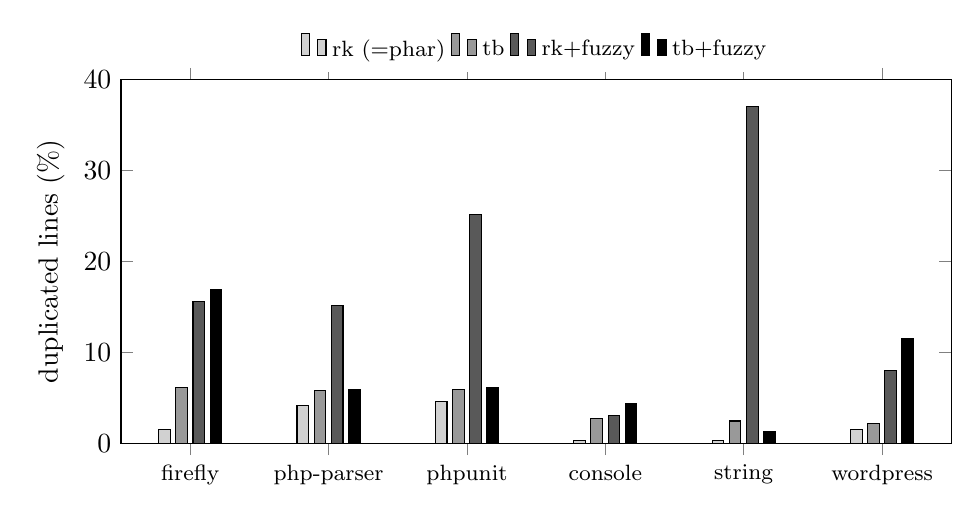
\begin{tikzpicture}
\begin{axis}[
  ybar,
  bar width=4.2pt,
  width=\textwidth, height=6.2cm,
  enlarge x limits=0.10,
  ymin=0, ymax=40,
  ylabel={duplicated lines (\%)},
  symbolic x coords={firefly,php-parser,phpunit,console,string,wordpress},
  xtick=data,
  x tick label style={font=\footnotesize},
  ytick={0,10,20,30,40},
  legend style={at={(0.5,1.02)},anchor=south,legend columns=4,font=\footnotesize,draw=none},
]
\addplot+[ybar,fill=g4,draw=black] coordinates {(firefly,1.54)(php-parser,4.15)(phpunit,4.64)(console,0.27)(string,0.33)(wordpress,1.51)};
\addplot+[ybar,fill=g3,draw=black] coordinates {(firefly,6.09)(php-parser,5.81)(phpunit,5.89)(console,2.73)(string,2.45)(wordpress,2.18)};
\addplot+[ybar,fill=g2,draw=black] coordinates {(firefly,15.58)(php-parser,15.13)(phpunit,25.15)(console,3.04)(string,37.07)(wordpress,7.97)};
\addplot+[ybar,fill=g1,draw=black] coordinates {(firefly,16.88)(php-parser,5.93)(phpunit,6.17)(console,4.40)(string,1.33)(wordpress,11.47)};
\legend{rk (=phar), tb, rk+fuzzy, tb+fuzzy}
\end{axis}
\end{tikzpicture}
\caption{Duplicated-line percentage by algorithm variant across six corpora.
\texttt{rk} reproduces the original phar exactly; \texttt{tb} adds a controlled increment
(reordered blocks); \texttt{-{}-fuzzy} variants inflate the reported rate (up to 37\% on \texttt{symfony/string}),
which is why fuzzing is a hidden research flag, not a default.}
\label{fig:compare}
\end{figure}

\begin{table}[h]
\centering
\caption{Duplicated-line \% per corpus and variant. \texttt{rk} matches the original phar to two
decimals on every corpus (100\% backward compatibility).}
\label{tab:compare}
\small
\begin{tabular}{l rrrrr}
\toprule
\textbf{corpus} & \textbf{phar/rk} & \textbf{rk+fuzzy} & \textbf{tb} & \textbf{tb+fuzzy} \\
\midrule
firefly-iii      & 1.54  & 15.58 & 6.09 & 16.88 \\
php-parser       & 4.15  & 15.13 & 5.81 & 5.93 \\
phpunit          & 4.64  & 25.15 & 5.89 & 6.17 \\
symfony-console  & 0.27  & 3.04  & 2.73 & 4.40 \\
symfony-string   & 0.33  & 37.07 & 2.45 & 1.33 \\
wordpress        & 1.51  & 7.97  & 2.18 & 11.47 \\
\bottomrule
\end{tabular}
\end{table}

\paragraph{Findings.} (1)~\texttt{rk} equals the original phar on every corpus --- 100\% backward
compatibility. (2)~\texttt{rk+fuzzy} is unsuitable as a default: $3$--$80\times$ the baseline with
near-zero precision gain. (3)~\texttt{tb} is the best complement to \texttt{rk}: it adds the
reordered clones \texttt{rk} misses while staying within $1.5$--$4\times$ the baseline, kept precise
by the IDF filter. (4)~\texttt{tb+fuzzy} is corpus-dependent and not a safe default.
(5)~the suffix tree, even after the banded-DP optimization below cut its matching cost
$\sim$3.5$\times$, stays above interactive speed on corpora over a few hundred files, so it is retained
for targeted studies, not the default. Read together, these place \texttt{rk+fuzzy} as a dominated
configuration --- its volume increase is inferred false positives, consistent with the dominance
result of \S\ref{sec:eval} --- and \texttt{rk+tb} as the non-dominated choice on the precision--cost
frontier; because the six public corpora carry no labelled recall, we claim consistency with that
frontier rather than optimality on it.

\paragraph{Optimizing the suffix tree.} Rather than adopt plausible but untargeted advice (object-free
node storage and Ukkonen construction, both already present), we profiled. Construction is $O(n)$ and
negligible; the approximate-matching edit-distance DP accounts for roughly 70\% of \texttt{findClones}
and grows super-linearly with \texttt{maxErrors}. By the band-sufficiency lemma (\S\ref{sec:methods}),
the full $O(L^2)$ matrix is unnecessary: restricting computation to the diagonal band of width
$2\,\texttt{maxErrors}+1$ (the Ukkonen cutoff) lowers it to $O(L\cdot\texttt{maxErrors})$ with identical
output. On a Firefly~III slice this reduced \texttt{findClones} by
$\sim$3.5$\times$ at every edit distance with byte-identical clone output; the residual cost is
candidate enumeration, which banding does not address. The change was admitted only after the benchmark
confirmed unchanged results --- the same evidence-before-adoption rule applied throughout.

\paragraph{Default mode.} \texttt{phpcpd <dir>} now runs \textbf{rk\,+\,tb combined} (exact $+$
reorder-tolerant, merged with deduplication); \texttt{-{}-rk} restricts to Rabin--Karp only. Research
flags (\texttt{-{}-fuzzy}, \texttt{-{}-algorithm}, \texttt{-{}-edit-distance}, \dots) remain
parseable but hidden from \texttt{-{}-help} to prevent accidental production use
(Table~\ref{tab:reco}).

\begin{table}[h]
\centering
\caption{Recommended invocation by goal.}
\label{tab:reco}
\small
\begin{tabular}{l l l}
\toprule
\textbf{Goal} & \textbf{Command} & \textbf{Output} \\
\midrule
Daily DRY check       & \texttt{phpcpd src/}                       & rk+tb, clean signal \\
Exact clones (CI speed)& \texttt{phpcpd -{}-rk src/}               & matches original phar \\
Type-3 gapped study   & \texttt{phpcpd -{}-algorithm suffixtree src/} & small/medium repos \\
Type-2 research       & \texttt{phpcpd -{}-algorithm tokenbag -{}-fuzzy src/} & high recall, low prec. \\
\bottomrule
\end{tabular}
\end{table}

\section{Evaluation: BCB-PHP}
\label{sec:eval}

\subsection{BCB-PHP: a labelled PHP clone benchmark}
A study of clone-detection methods needs labelled ground truth, and for PHP none existed: the standard
benchmarks are language-bound --- BigCloneBench~\cite{bigclonebench} is Java, POJ-104 is C --- leaving
PHP with no equivalent. Without one, the methods of \S\ref{sec:methods}--\ref{sec:engineering} could
be implemented but not honestly compared. We therefore built \textbf{BCB-PHP}: a mutation-injection
harness that generates ground-truth Type-1/2/3 variants from real PHP across a curated, pinned corpus,
following SourcererCC's injection-based ground-truth approach~\cite{sourcerercc}. To respect corpus
licences (WordPress GPLv2, Firefly~III AGPLv3, the rest permissive) the released artifact is a
fetch-script $+$ commit SHAs $+$ injection manifests $+$ harness --- never redistributed source.

Building the benchmark is a contribution in its own right, and we release it for reuse. Its corpora
span a deliberate type-density gradient (\S\ref{sec:typedensity}), from traditional untyped PHP
(WordPress) to PHPStan/Larastan-max typed codebases (PHPUnit, Firefly~III). That axis lets others
study questions this paper only begins to answer: how clone detection behaves on \emph{modern typed}
versus \emph{traditional untyped} PHP, and how detection methods differ from one another on the same
labelled inputs.

\subsection{Type-density is the independent variable}
\label{sec:typedensity}
The thesis ``type information improves clone detection'' is proved not by one typed corpus but by
showing detection quality as a function of \emph{how typed} the code is. Corpus type-density is thus
the experiment's $x$-axis and untyped code is the control end of it.

\defn{signature type-density}
$\mathrm{td} = (\text{typed signature slots}) / (\text{total signature slots})$, where slots are
function/method parameters and return-type positions. The signature surface is unambiguously
tokenizable; property declarations are excluded to avoid guessing class context.

We compute the map rather than assert it (Figure~\ref{fig:scatter}, Table~\ref{tab:density}).
Clone-density is measured by the Rabin--Karp engine, independent of the type axis. The predictions
hold: WordPress anchors the untyped end (13.3\%), the PHPStan/Larastan-max codebases (PHPUnit 92.7\%,
Firefly~III 90.7\%) the typed end, with a clean spread between --- a usable axis, not a hunch.

\begin{figure}[h]
\centering
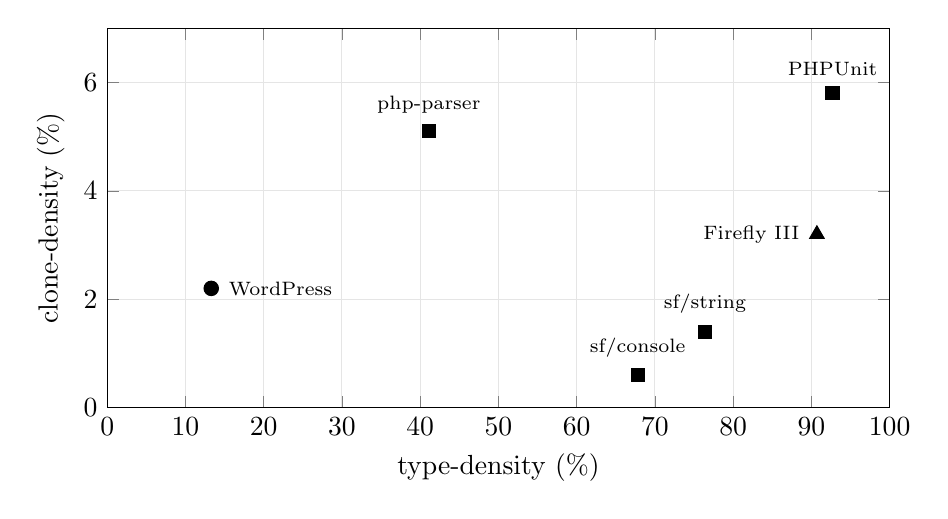
\begin{tikzpicture}
\begin{axis}[
  width=0.95\textwidth, height=6.4cm,
  xlabel={type-density (\%)}, ylabel={clone-density (\%)},
  xmin=0, xmax=100, ymin=0, ymax=7,
  grid=both, grid style={black!10},
  every node near coord/.append style={font=\scriptsize, anchor=south},
]
\addplot[only marks, mark=*,        mark size=2.6pt, black] coordinates {(13.3,2.2)};
\addplot[only marks, mark=square*,  mark size=2.4pt, black] coordinates {(41.1,5.1)(67.8,0.6)(76.4,1.4)(92.7,5.8)};
\addplot[only marks, mark=triangle*,mark size=3.0pt, black] coordinates {(90.7,3.2)};
\node[anchor=west,font=\scriptsize] at (axis cs:14.3,2.2) {WordPress};
\node[anchor=south,font=\scriptsize] at (axis cs:41.1,5.25) {php-parser};
\node[anchor=south,font=\scriptsize] at (axis cs:67.8,0.75) {sf/console};
\node[anchor=south,font=\scriptsize] at (axis cs:76.4,1.55) {sf/string};
\node[anchor=east,font=\scriptsize] at (axis cs:89.7,3.2) {Firefly III};
\node[anchor=south,font=\scriptsize] at (axis cs:92.7,5.95) {PHPUnit};
\legend{}
\end{axis}
\end{tikzpicture}
\caption{Type-density $\times$ clone-density map (full corpora, pinned SHAs).
Marks: $\bullet$~untyped control, $\blacksquare$~injection substrate,
$\blacktriangle$~ecological corpus. The scarce typed-and-cloney quadrant is occupied by an
application (Firefly~III), not a library.}
\label{fig:scatter}
\end{figure}

\begin{table}[h]
\centering
\caption{Computed type-density / clone-density map (\texttt{bench/measure-density.php}).}
\label{tab:density}
\small
\begin{tabular}{l r r r l}
\toprule
\textbf{corpus} & \textbf{files} & \textbf{type-dens.} & \textbf{clone-dens.} & \textbf{bucket} \\
\midrule
WordPress          & 1889 & 13.3\% & 2.2\% & untyped control \\
\texttt{nikic/php-parser} & 341 & 41.1\% & 5.1\% & injection (dependency) \\
\texttt{symfony/console} & 359 & 67.8\% & 0.6\% & injection \\
\texttt{symfony/string} &  33 & 76.4\% & 1.4\% & injection \\
Firefly III        & 1446 & 90.7\% & 3.2\% & ecological \\
PHPUnit            & 2699 & 92.7\% & 5.8\% & injection (reflexive) \\
\bottomrule
\end{tabular}
\end{table}

\subsection{E2 --- the effect of type information}
The decisive operator, possible only in typed PHP, clones a block and changes an \texttt{int}-typed
variable to \texttt{string}-typed with structure held identical. Name-blind normalization calls these
clones (false positive); type-anchored normalization (\texttt{-{}-type-anchored}, which preserves
built-in type keywords instead of folding them to \texttt{ID}) correctly separates them. Injecting at
\emph{function} granularity over the full eligible population (functions carrying an
\texttt{int}/\texttt{float} hint, $\ge 25$ tokens), Figure~\ref{fig:lift} and Table~\ref{tab:e2}
report specificity.

\begin{figure}[h]
\centering
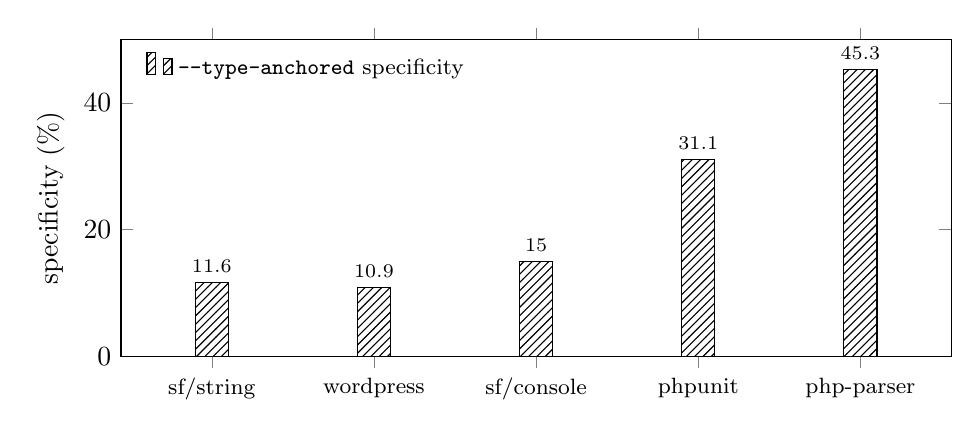
\begin{tikzpicture}
\begin{axis}[
  ybar,
  bar width=12pt,
  width=\textwidth, height=5.6cm,
  enlarge x limits=0.14,
  ymin=0, ymax=50,
  ylabel={specificity (\%)},
  symbolic x coords={sf/string,wordpress,sf/console,phpunit,php-parser},
  xtick=data,
  x tick label style={font=\footnotesize},
  nodes near coords, nodes near coords align={vertical},
  every node near coord/.append style={font=\scriptsize, text=black},
  legend style={at={(0.02,0.98)},anchor=north west,font=\footnotesize,draw=none},
]
\addplot+[ybar,pattern=north east lines,pattern color=black,draw=black] coordinates {(sf/string,11.6)(wordpress,10.9)(sf/console,15.0)(phpunit,31.1)(php-parser,45.3)};
\legend{\texttt{-{}-type-anchored} specificity}
\end{axis}
\end{tikzpicture}
\caption{Specificity on same-shape-different-type pairs. Name-blind \texttt{-{}-fuzzy} is a flat 0\%
floor (it calls every such pair a clone, so it is omitted from the bars); \texttt{-{}-type-anchored}
lifts specificity by $+10.9$ to $+45.3$ points at \emph{zero} recall cost (recall $=100\%$ in both
modes, Table~\ref{tab:e2}).}
\label{fig:lift}
\end{figure}

\begin{table}[h]
\centering
\caption{E2: type-anchored normalization over the full eligible-function population. Recall is identical in both modes;
the lift is pure specificity gain.}
\label{tab:e2}
\small
\begin{tabular}{l r r r r c}
\toprule
\textbf{corpus} & \textbf{fns} & \makecell{\textbf{spec.}\\\textbf{fuzzy}} &
\makecell{\textbf{spec.}\\\textbf{anchored}} & \textbf{lift} & \textbf{recall} \\
\midrule
\texttt{symfony/string}  &  43 & 0.0\% & 11.6\% & $+11.6$ & $100\%$ \\
\texttt{symfony/console} & 100 & 0.0\% & 15.0\% & $+15.0$ & $100\%$ \\
PHPUnit                  & 122 & 0.0\% & 31.1\% & $+31.1$ & $100\%$ \\
\texttt{nikic/php-parser}& 128 & 0.0\% & 45.3\% & $+45.3$ & $100\%$ \\
WordPress                &  55 & 0.0\% & 10.9\% & $+10.9$ & $100\%$ \\
\bottomrule
\end{tabular}
\end{table}

The lift is a property of \emph{type-load-bearing} functions, not of corpora: php-parser shows the
largest lift despite mid type-density because its small node/visitor methods are dominated by their
typed signatures, whereas WordPress's few typed functions are large and procedural. The corpus-level
benefit therefore scales with type-density (Figure~\ref{fig:scatter}), which is why the per-corpus
story needs \emph{two} figures, not one. Because the two modes share the same recall, this is a clean
dominance relation: on same-shape-different-type pairs, type-anchored normalization
\emph{Pareto-dominates} name-blind fuzzing --- equal recall at strictly higher specificity --- the
strongest form the claim can take, since here both axes are measured against injected ground truth.

\subsection{E3 --- inconsistent clones in practice}
\texttt{bench/run-e3.php} scans the ecological corpus (Firefly~III, 200 most-recently-modified files)
once through the suffix tree (\texttt{-{}-algorithm suffixtree -{}-edit-distance 3 -{}-min-tokens 50}), reads
the gapped clones via \lstinline!CodeClone::isGapped()! (the R4 capability), deduplicates by file
pair, and cross-references git: the \emph{staleness gap} is the number of days between the two copies'
last commits --- a high gap means one copy was maintained long after its sibling, the canonical
inconsistent-clone risk. The scan found 68 inconsistent clones and two distinct diverged-copy pairs
(Table~\ref{tab:e3}); both were manually verified as real. Exact-match output (Rabin--Karp /
\texttt{-{}-rk}) flags neither as inconsistent, having no gapped-clone concept.

\begin{table}[h]
\centering
\caption{E3 diverged-copy pairs in Firefly~III (200-file slice), ranked by staleness. Both verified
manually against source.}
\label{tab:e3}
\footnotesize
\begin{tabular}{@{}c p{2.6cm} p{2.6cm} c c p{4.0cm}@{}}
\toprule
\textbf{\#} & \textbf{copy A} & \textbf{copy B} & \textbf{lines} & \textbf{stale (d)} & \textbf{verdict} \\
\midrule
1 & \texttt{Navigation\-AddPeriodTest} & \texttt{Navigation\-PreferredSql\-FormatTest} & 4 & 35 &
Real --- duplicated \lstinline!setUp()! scaffold across two tests of the same class; a shared base
would remove it. \\
2 & \texttt{Autocomplete/\-CurrencyController} & \texttt{Autocomplete/\-TagController} & 25 & 9 &
Real --- identical DI constructor $+$ search loop; \texttt{Currency} later gained a deprecated
endpoint \texttt{Tag} never received. \\
\bottomrule
\end{tabular}
\end{table}

\section{Availability}
phpcpd-next is openly available under the permissive BSD~3-Clause licence, retaining the upstream
copyright of Sebastian Bergmann. It has zero runtime dependencies (\texttt{php >=8.5} plus
\texttt{ext-dom}/\texttt{ext-mbstring}) and projects one format-neutral model
(\lstinline!CodeCloneMap!) to Text, PMD-CPD XML, JSON, and SARIF~2.1.0 --- the last ingested natively
by GitHub Code Scanning, with gapped (inconsistent) clones emitted at \texttt{warning} severity and
exact clones at \texttt{note}, so the bug-bearing clones surface as higher-severity PR annotations.
BCB-PHP ships as a fetch-script $+$ pinned SHAs $+$ injection manifests $+$ harness; every result is
reproducible from the SHAs and \texttt{composer.lock} files, and the modernization is recorded
diff-by-diff in \texttt{MODERNIZATION.md}.

\section{Conclusion}
Starting from \texttt{phpcpd}'s Rabin--Karp exact matcher and its unreleased suffix-tree engine, we
asked an empirical question: of the clone-detection methods available, which are appropriate for a fast
PHP tool? Answering it required infrastructure that did not exist --- a labelled PHP clone benchmark ---
so we constructed one (BCB-PHP) while modernizing and completing the inherited engines and implementing
additional literature-grounded methods. The results --- a type-density gradient, a $+10.9$ to $+45.3$
point specificity increase from type-aware normalization at no recall cost, a six-corpus method
comparison, and confirmed inconsistent clones in an application corpus --- support a default that
combines exact and reorder-tolerant matching (\texttt{rk+tb}), retains fuzzing only for research, and
reserves approximate suffix-tree matching for targeted analysis.

\paragraph{Future work.} The component most likely to outlast any single result is the benchmark, since
it turns open questions about PHP clone detection from matters of argument into measurable ones. Three
directions follow from the evidence. First, the injection operators can be broadened beyond the
\texttt{int}/\texttt{float} confusion studied here to a wider class of type-level edits
(\texttt{bool}$\leftrightarrow$\texttt{int}, nullable versus non-nullable, and class or interface
substitutions), enlarging the type-load-bearing population and testing whether the specificity gain of
type-anchored normalization generalizes across type kinds. Second, the harness can be applied to
further real-world and proprietary codebases to assess external validity beyond the six public corpora.
Third, the residual cost of suffix-tree matching --- candidate enumeration, the part the banded DP
(\S\ref{sec:practical}) does not reduce --- remains the engine's main scaling limit on large corpora
and is the natural next optimization, again gated on benchmark-validated, output-preserving change. In each case the methodological commitment is the
one adopted throughout: a candidate improvement is admitted on PHP-specific empirical evidence, not on
its theoretical appeal.

\begin{thebibliography}{99}
\small
\bibitem{roycordy} C.~K. Roy and J.~R. Cordy, ``A survey on software clone detection research,''
Queen's Univ.\ Tech.\ Rep.\ 2007-541, 2007.

\bibitem{conqat} E.~Juergens, F.~Deissenboeck, B.~Hummel, and S.~Wagner, ``Do code clones matter?''
in \emph{Proc.\ ICSE}, 2009, pp.~485--495.

\bibitem{sourcerercc} H.~Sajnani, V.~Saini, J.~Svajlenko, C.~K. Roy, and C.~V. Lopes,
``SourcererCC: scaling code clone detection to big-code,'' in \emph{Proc.\ ICSE}, 2016,
pp.~1157--1168. arXiv:1512.06448, 1603.01661.

\bibitem{toma} Y.~Wu \emph{et al.}, ``Toma: a token-type-aware clone detector'' (token-type
abstraction, six similarity measures, ``simple clones dominate''), in \emph{Proc.\ ICSE}, 2024.

\bibitem{hummel} B.~Hummel, E.~Juergens, L.~Heinemann, and M.~Conradt, ``Index-based code clone
detection: incremental, distributed, scalable,'' in \emph{Proc.\ ICSM}, 2010, pp.~1--9.

\bibitem{deckard} L.~Jiang, G.~Misherghi, Z.~Su, and S.~Glondu, ``DECKARD: scalable and accurate
tree-based detection of code clones,'' in \emph{Proc.\ ICSE}, 2007, pp.~96--105.

\bibitem{bigclonebench} J.~Svajlenko, J.~F. Islam, I.~Keivanloo, C.~K. Roy, and M.~M. Mia,
``Towards a big data curated benchmark of inter-project code clones,'' in \emph{Proc.\ ICSME}, 2014,
pp.~476--480.
\end{thebibliography}

\end{document}
